The CBGB apparatus design has various stages, a room temperature 300 K outer aluminum vacuum chamber, onto which a Pulse Tube Refrigerator (PTR) is mounted, an aluminum radiation shield mounted to the 40 K PTR cooling stage, and an inner copper cryopumping shield and experimental cell connected to the 4 K PTR cooling stage. Connected to the vertical vacuum chamber, a "stem" region protrudes out from the beam side, as seen in Figures \ref{fig: SW chamber} and \ref{fig: chamber}, where a large Agilent Varian-V 551 turbo pump evacuates the entire volume. The beam comes out of the experimental cell and shield, through a set of apertures, into the stem region where skimmers and shutters are mounted to manipulate the beam.

A Cryomech PT415 PTR with a remote head option was attached to the top plate of the vacuum chamber with a large bellows mount to isolate the chamber from the mechanical vibrations caused by the PTR motor head. The chamber was pumped down to normal operating pressures, where then 4 retaining screws were tightened to just above the bellow's compressed height. This maintains mechanical decoupling between the outer vacuum chamber and the PTR while running.

We want to minimize the mechanically coupling onto the PTR due to the fragility of the pulse tube walls; small amounts of force applied onto a mechanically connected component would risk torquing the walls to break. Thus, all components inside the CBGB are mechanically connected to the top plate of the vacuum chamber via 8-32 stainless steel (SS316) threaded rods. Thermal connections are made with copper braids welded onto L-shaped brackets that mount between platforms secured to the PTR cooling stages, and the shields.

Not only are all the inner shields connected to the top plate, but so are the feedthroughs including gas fill lines. This ensures that any and all connections made into the CBGB are not disturbed when opening the outer vacuum chamber to expose the inner components.

The design of the shields themselves is informed by the choice of buffer gas species. Commonly used buffer gas species are helium and neon, while helium provides a slower beam, it is more technically challenging to implement. The main technical difference comes from the cryopumping requirements; where neon only needs surfaces to be held at 17 K to continually cryopump, helium requires (coconut) activated charcoal held at 4 K or lower. Aside from the difficulty of getting surfaces to 4 K these volumes of charcoal can become saturated and require purging, limiting one's operating time (few hours). On the other hand, neon ice formed on the 17 K surface will act as a cryopump for more neon gas, allowing for many hours of continuous operation with no appreciable build up of background gas. Our experiment uses neon as a buffer gas for its technical simplicity, the lower achievable temperature with the helium does not yield dramatic gains in the final reaction temperature.

\begin{figure}[H]
	\centering
	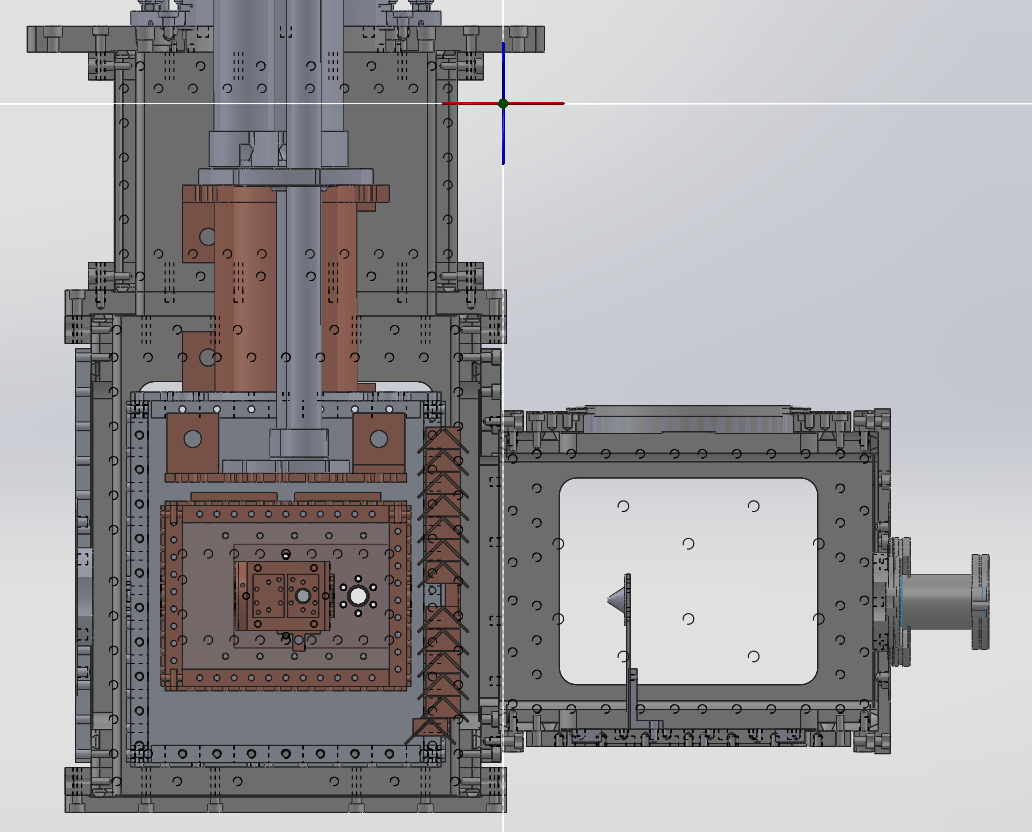
\includegraphics[width=1\textwidth]{images/CBGB_solidworks_cross_section.png}
	\caption{Cross sectional view of CBGB in solidworks. Components include copper sheath for PTR, aluminum radiation shield with chevron baffles, copper shield and experimental cell, and skimmer mounted in stem chamber. The baffles allow for gas to flow into the cold region of the beam apparatus, while preventing 300 K black body radiation from hitting the inner shield and cell.}
	\label{fig: SW chamber}
\end{figure}

\begin{figure}[H]
	\centering
	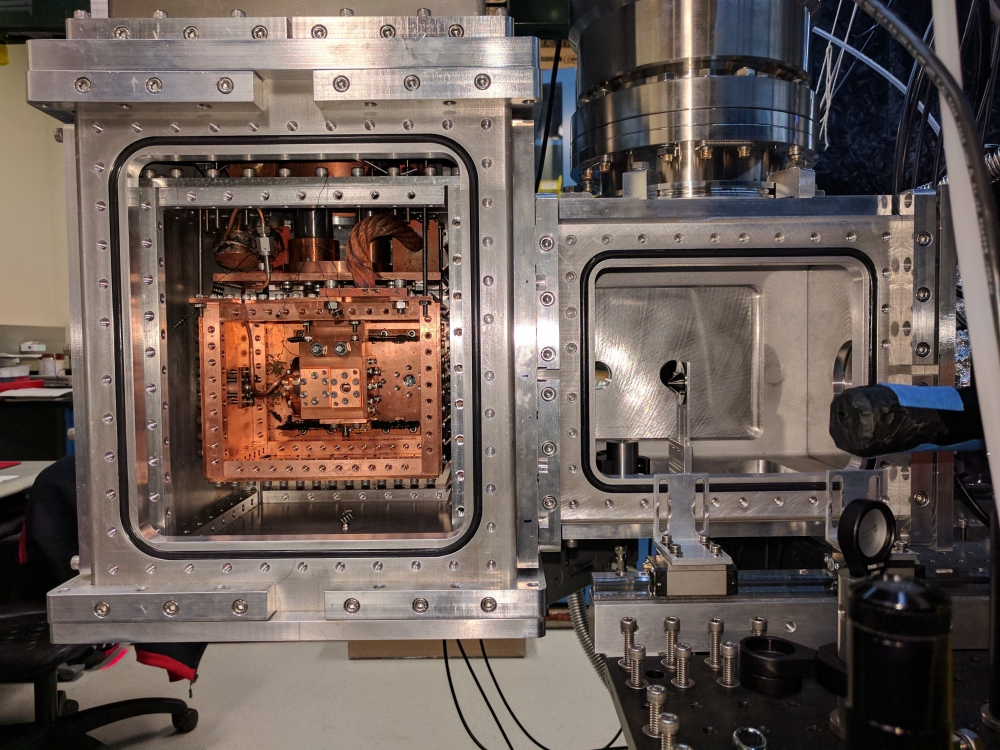
\includegraphics[width=1\textwidth]{images/CBGB_cross_section.jpg}
	\caption{Cross sectional view of CBGB with side walls removed from the outer vacuum chamber, 40 K aluminum radiation shield, and inner 4 K cryopumping shield exposing the inner experimental cell. A skimmer is mounted in the stem region.}
	\label{fig: chamber}
\end{figure}